\documentclass[t]{beamer}
\usepackage{CJKutf8}
\usepackage{amsfonts}
    \usepackage{amsmath}
    \usepackage{amssymb}
    \usepackage{amsthm}
    \usepackage{enumerate}
    \usepackage{graphicx}
    \usepackage{layout}
    \usepackage{mathrsfs}
    \usepackage{fancyhdr}
    \usepackage{subfigure}
    \usepackage{tcolorbox}
    \usepackage{tikz-cd}
    \usepackage{color}
    \usepackage{pifont}
    \usepackage{verbatim}
    \usepackage{mathtools}
    \usepackage{float}
    \usepackage{bm}
    \usetheme{AnnArbor}
% \usetheme{Antibes}
\usecolortheme{beaver}

% 添加网址的命令
\usepackage{hyperref}
% 这是一个带链接文本的示例:\href{https://www.example.com}{点击这里访问网站}
% 普通的示例:\url{https://www.example.com}
% 表格
\usepackage{booktabs}
\usepackage{multirow}

% \setbeamertemplate{navigation symbols}{}

\usepackage{textpos}

\newcommand{\dif}{\mathrm{d}}
\newtheorem{thm}{{定理}}

% some common command
\newcommand{\mm}[1]{$ #1$\newline}
% \newcommand{\tuichu}{\Rightarrow}
% \newcommand{\li}[1]{\newline#1}



\newcommand{\analysis}[2]{\forall \mathcal{E}{#1},\exists \delta {#2},s.t.}
\newcommand{\denyanalysis}[2]{\exists \mathcal{E}{#1},\forall \delta {#2},s.t.}
\newcommand{\yield}{\Rightarrow }
\newcommand{\jj}{\newline}
\newcommand{\ff}[1]{$ #1$}   % math environment + newline
\newcommand{\fgn}[1]{\begin{equation}#1\end{equation}  }
\newcommand{\fg}[1]{$$ #1$$}   % math environment + newline 
\newcommand{\pf}{$proof.$\newline}
\newcommand{\ee}{\newline\ff{\Box}\newline}
\newcommand{\fenshi}[2]{\ff{\frac{#1}{#2}}}
\newcommand{\shenlue}{\vdots\jj}
\newcommand{\abs}[1]{{\left \lvert #1 \right\rvert}}
\newcommand{\loge}[1]{In ({#1})}
\newcommand{\logical}[2]{log_{#2}^{#1}}
\newcommand{\summary}[3]{$\sum_{{#1}={#2}}^{#3}  $}
\newcommand{\denjia}[2]{{#1}\Leftrightarrow {#2}}
\newcommand{\jihe}[3]{ {#1}  = \{ {#2} \mid {#3} \} }
\newcommand{\ve}[2]{\left\langle {#1},{#2}\right \rangle}
\newcommand{\dakuohao}[2]{\begin{array}{rcl}{#1}\end{array} \} \Rightarrow{#2}}
\newcommand{\sxb}[3]{#1^{#2}_{#3}}
\newcommand{\sss}[2]{#1^{#2}}
\newcommand{\xxx}[2]{#1_{#2}}
\newcommand{\bri}[1]{\uppercase\expandafter{\romannumeral#1}}
\newcommand{\ri}[1]{\romannumeral#1} 
\newcommand{\polynomial}[8]{#1_{#2}#6^{#7}+#1_{#3}#6^{#8}+...+#1_{#4}#6+#1_{#5} }
\newcommand{\newd}[4]{f[{#1}_{#2},{#4},{#1}_{#3}]}
\newcommand{\lb}[2]{\begin{align*}\begin{split}{#1}\{ {#2}\end{split}\end{align*}}
\newcommand{\tab}[1]{\begin{array}{ll} {#1}\end{array}}


% 向量乘积
\newcommand{\avg}[1]{\left\langle #1 \right\rangle}
% 偏微分方程
\newcommand{\difFrac}[2]{\frac{\dif #1}{\dif #2}}
\newcommand{\pdfrac}[2]{\frac{\partial{#1}}{\partial{#2}}}
% 不同章节
\newcommand{\one}[1]{\section{#1}}
\newcommand{\two}[1]{\subsection{#1}}
\newcommand{\three}[1]{\subsubsection{#1}}
\newcommand{\aone}[1]{\section*{#1}}
\newcommand{\atwo}[1]{\subsection*{#1}}
\newcommand{\athree}[1]{\subsubsection*{#1}}
% 大括号,左右都有
\newcommand{\lbra}[1]{\left\{  {\begin{matrix} #1 \end{matrix}}\right. } 
% 样式 括号前缀 + 括号 
\newcommand{\lbras}[2]{{#1}\left\{ {  {\begin{matrix} #2 \end{matrix}}}\right. } 
\newcommand{\rbra}[1]{ \left.  {\begin{matrix} #1 \end{matrix}} \right\}  } 
% 模长
\newcommand{\distance}[1]{\parallel #1\parallel }
% 等价
\newcommand{\equ}{\Longleftrightarrow }
% 共轭
\newcommand{\cja}[1]{\overline{#1}}
% 两个矩阵,上面是 方框[] 下面是线条| 中间是 无
\newcommand{\mtx}[1]{\begin{matrix}#1\end{matrix} }
\newcommand{\bmtx}[1]{\begin{bmatrix}#1\end{bmatrix} }
\newcommand{\vmtx}[1]{\begin{vmatrix}#1\end{vmatrix} }
% \newcommand{\table}[1]{\begin{array}[lr]{ccc} #1 \end{array}}

%输入普通字符
\newcommand{\ww}[1]{\text{#1}}

% 所有内容 直接头文件搞定
\newcommand{\everything}[1]{\begin{document}\begin{CJK*}{UTF8}{gkai}#1\end{CJK*}\end{document}}


% 存放代码(失败了)
\newcommand{\cccode}[1]{\begin{lstlisting}#1\end{lstlisting}}

% 改变特定行序列
\newcommand{\ttt}{\subsection{}}

% 嵌套序号
\newcommand{\eee}[1]{\begin{enumerate}#1\end{enumerate}}


% 模板里面的一些宏
\newcommand{\pdfFrac}[2]{\frac{\partial #1}{\partial #2}}
\newcommand{\OFL}{\mathrm{OFL}}
\newcommand{\UFL}{\mathrm{UFL}}
\newcommand{\fl}{\mathrm{fl}}
\newcommand{\op}{\odot}
\newcommand{\Eabs}{E_{\mathrm{abs}}}
\newcommand{\Erel}{E_{\mathrm{rel}}}
% 变化颜色
\newcommand{\red}{\textcolor{red}}
\newcommand{\blue}{\textcolor{blue}}



% 流程图需要用到的宏包
\usepackage{palatino}
\usepackage{tikz}
\usetikzlibrary{shapes.geometric, arrows}
\tikzstyle{startstop} = [rectangle, rounded corners, minimum width = 2cm, minimum height=1cm,text centered, draw = black, fill = red!40]
\tikzstyle{io} = [trapezium, trapezium left angle=70, trapezium right angle=110, minimum width=2cm, minimum height=1cm, text centered, draw=black, fill = blue!40]
\tikzstyle{process} = [rectangle, minimum width=3cm, minimum height=1cm, text centered, draw=black, fill = yellow!50]
\tikzstyle{decision} = [diamond, aspect = 3, text centered, draw=black, fill = green!30]
% 箭头形式
\tikzstyle{arrow} = [->,>=stealth]
% 4个非常重要 的新命令
\newcommand{\start}[2]{    \node (start) [startstop]{#1};\node (in1) [io, below of = start]{#2};\lin{start}{in1}{}}
\newcommand{\stopp}[3]{\node (out1) [io, below of= #1]{#2};\node (stop) [startstop, below of=out1]{#3};\lin{out1}{stop}{} }
\newcommand{\pro}[6]{    \node (#3) [process, #2 of=#1,xshift=#4 cm]{#5};}
\newpage
\newcommand{\lin}[3]{\draw [arrow] (#1) --node [above] {#3} (#2);}


\begin{document}
\begin{CJK*}{UTF8}{gkai}
% 一般第一页显示PPT标题以及作者信息

% \BackgroundPic{./Screenshot from 2022-04-20 16-31-08.png}

% 增加学校 前面
\addtobeamertemplate{title page}{}{
	\begin{tikzpicture}[remember picture,overlay]
		% \node[yshift=85pt,xshift=50pt]{\includegraphics[height=2cm]{Screenshot from 2022-04-20 16-51-21.png}};
\end{tikzpicture}
}


	\title{创建时间序列的指令微调的数据集合并进行微调}
	\subtitle {} %不需要
	\author{
		陈钶杰\, \\
		专业:计算数学\,
	} % 显示作者
	% \institute {学院:数学科学学院} % 设置学院机构	
	\date{\today}  % 显示日期
\titlepage

% 设置目录
\begin{frame}{目录}
\frametitle{目录}	
\tableofcontents  % 显示目录
\end{frame} 



\section{论文解读-具有内存的大型语言模型(LLM)在计算机上是通用的}  

\begin{frame}
	\frametitle{}
		\textcolor{red}{摘要}
		\begin{itemize}
		\item 论文摘要指出,传统的神经记忆机制无法支持 LLM 模拟复杂推理,该论文提议使用数据库作为 LLM 的新型符号存储器,以增强其推理能力。拟议的名为ChatDB的框架使用内存链方法来更有效地操作外部符号存储器,从而可以有效地操作内存和处理复杂的多表数据库交互,从而提高准确性和稳定性。
		% \item 符号存储器:比如c++里面的x=10,y=5,这里的x和y都是符号存储器的意思。变量x,y在程序中被用作存储和引用数据的标识符。通过给个符号名称,我们可以在程序的不同部分引用和操纵这些数据,而无需直接操作内存地址。
		% \item SQL数据库:它以表格的形式组织和存储数据,并提供了一种标准化的方式来查询、操作和管理这些数据。
		\end{itemize}
\end{frame}

\begin{frame}
	\frametitle{introduction}
		\eee{
			\item 本文涵盖了使用实例化为 LLM 的符号内存框架和一组 SQL 数据库,使用符号内存增强大型语言模型 (LLM) 以实现复杂的多跳推理。本文讨论了LLM的局限性,并提出了一种名为ChatDB的框架,该框架通过实验进行了评估,结果证明其性能优于基准模型ChatGPT。本文还讨论了ChatDB与现有方法相比的独特特性和功能,重点介绍了使用符号存储器增强LLM的优势。
			\item 本文的重点是用数据库形式的符号记忆来增强LLM,以增强复杂的推理。
		}
\end{frame}

\begin{frame}
	%  \frametitle{主要流程}
	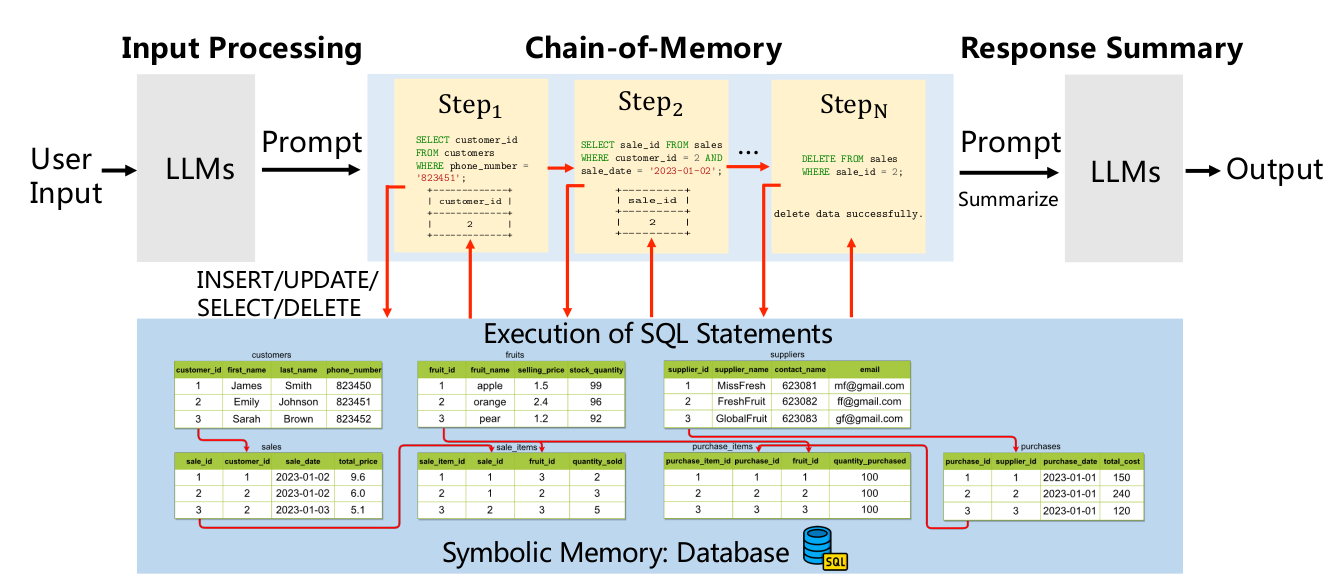
\includegraphics[scale=0.25]{png/process.png}
	\begin{itemize}
		\item input:手机号为823451的顾客在2023年1月2日买了什么东西?
		\item output:买了几个梨
		\item 说明:输入这段话以后,第一步模型尝试从所有顾客中根据手机号823451找出顾客的购物id号,第二步在销售号码中根据顾客的购物id号和购买日期得到销售号,...,通过一步一步有逻辑的推导得到最后的结果具体买了什么水果。
	\end{itemize}
\end{frame}


\begin{frame}
	\frametitle{相关工作}	
	\eee{
		\item 本文讨论了大型语言模型(LLM)领域的相关工作及其局限性。该论文指出,尽管具有内存的 LLM 在计算上是通用的,但主流 LLM 并没有充分利用内存。本文还讨论了使用内存增强LLM的现有方法,例如基于矩阵的内存和基于提示的内存,并强调了它们的局限性。本文提出了一种名为ChatDB的新方法,该方法使用符号内存来增强LLM并解决了现有方法的局限性。
		}
\end{frame}


\begin{frame}
	\frametitle{ChatDB框架}	
	\begin{itemize}
		\item ChatDB 框架旨在使用符号存储器增强大型语言模型 (LLM),用于复杂的多跳推理。该框架由三个主要阶段组成:输入处理、内存链和响应摘要。
		\eee{
		\item 输入处理:在此阶段,处理用户输入并将其转换为框架可以使用的结构化格式。对输入进行分析以识别相关的实体和关系,然后将其存储在符号存储器中。
		\item 记忆链:这个阶段涉及一系列思维链步骤,其中复杂的推理被分解为一系列中间步骤。符号存储器用于存储每个步骤的中间结果,可用于跟踪 LLM 的当前状态并提供高度的可解释性。该框架使用 SQL 数据库作为符号内存,从而实现精确的操作和计算。LLM 生成 SQL 指令,将计算任务委托给外部数据库,从而确保每个步骤的准确性并防止错误累积。
		\item 响应摘要:在此阶段,根据内存链步骤的结果生成对用户的最终响应。该框架总结了中间结果,并生成了易于理解和解释的回应。
		}
		\item 通过实验对ChatDB框架进行了评估,结果证明其性能优于基准模型ChatGPT。本文重点介绍了ChatDB与现有方法相比的独特特性和功能,强调了使用符号存储器增强LLM的优势。
	\end{itemize}
\end{frame}



\begin{frame}
	\frametitle{模型评估}
	本文通过实验进行了评估,以评估使用数据库作为符号存储器来增强LLM的有效性。
	\eee{
		\item 将ChatDB框架与基准模型ChatGPT进行了比较,实验结果表明,ChatDB的性能明显优于ChatGPT,突显了符号内存集成的优势。
		\item 本文还讨论了ChatDB与现有方法相比的独特特性和功能。
	}
\end{frame}

\begin{frame}
	\frametitle{本文的实际含义}
	\eee{
		\item 拟议的ChatDB框架可用于通过使用数据库形式的符号存储器来增强大型语言模型(LLM)的推理能力。 
		\item 使用符号存储器和内存链方法可以防止错误积累并实现准确可靠的操作,从而使所提出的方法适用于复杂的多跳推理任务。 
		\item 所提出的方法可以应用于各种自然语言处理(NLP)任务,例如问答、对话系统和文本生成,以提高其性能和准确性。 
		\item 拟议的方法还可以扩展到其他领域,例如计算机视觉和机器人技术,在这些领域,推理和记忆是智能系统的关键组成部分。 
		\item 拟议的方法可以激发对符号记忆和LLM整合的进一步研究,从而开发更先进、更有能力的人工智能系统。		
	}
\end{frame}

\begin{frame}
	\frametitle{本文使用的方法}
	\eee{
		\item ChatDB 框架的开发,该框架使用大型语言模型 (LLM) 和 SQL 数据库的组合来创建用于复杂的多跳推理任务的符号内存系统。 
		\item 内存链方法的实现,其中 LLM 生成 SQL 指令来操作外部数据库内存,从而实现准确可靠的操作并防止错误积累。 
		\item 对多个基准数据集和任务的拟议方法的评估,包括 LAMBADA 语言建模任务、WikiHop 和 MedHop 问答任务以及 CoQA 对话式问答任务。 
		\item 将提议的方法与现有方法(包括 GPT-3 中使用的基于提示的内存方法)进行比较,显示出性能和准确性方面的显著改进。 
		\item 未来几项与符号存储器和 LLM 的集成有关的工作的提案,包括研究其他符号语言的使用,探索更先进的数据库系统的使用,以及评估拟议方法在其他基准数据集和任务上的性能。
	}
\end{frame}

\begin{frame}
	\frametitle{本文的结果}
	\begin{itemize}
		\item 论文的结果表明,在包括 LAMBADA 语言建模任务、WikiHop 和 MedHop 问答任务以及 CoQA 对话式问答任务在内的多个基准数据集和任务中,拟议的 ChatDB 框架的性能优于现有方法,例如 GPT-3 中使用的基于提示的内存方法。实验结果表明,ChatDB的准确率非常高,这凸显了使用数据库作为符号存储器的优势。这种方法不仅可以防止错误积累,还可以增强LLM的多跳推理和精确计算能力。
	\end{itemize}
\end{frame}

\begin{frame}
	\frametitle{本文的结论}
	\eee{
		% \item 关于使用数据库作为 LLM 的新型符号存储器以增强其推理能力的提议。 
		% \item ChatDB 框架的开发,它使用内存链方法来更有效地操作外部符号内存,从而实现有效的内存操作和复杂的多表数据库交互处理,提高了准确性和稳定性。
		% \item 演示了拟议方法在多个基准数据集和任务上的有效性,表明与现有方法相比,性能有了显著改善。 
		% \item 未来几项与符号存储器和 LLM 的集成有关的工作的提案,包括研究其他符号语言的使用,探索更先进的数据库系统的使用,以及评估拟议方法在其他基准数据集和任务上的性能。
		\item 拟议的ChatDB框架以数据库的形式使用符号存储器增强了LLM,是增强复杂的多跳推理任务的有效方法。使用符号内存和内存链方法可防止错误累积,并实现准确可靠的操作。
		\item 实验结果表明,在多个基准数据集和任务中,ChatDB 的性能优于现有方法,例如 GPT-3 中使用的基于提示的内存方法。
		\item 作者建议,未来的工作应研究其他符号语言的使用,探索更先进的数据库系统的使用,并评估拟议方法在其他基准数据集和任务上的性能。
	}
\end{frame}



% \begin{frame}
% 	\frametitle{评估}
% 	% \textcolor{red}{仔细区分这些不同的人机接口}	
% 		评估在本节中,我们进行实验来评估使用数据库作为其符号记忆来增强LLM的有效性。我们的实验结果表明,ChatDB显著优于基线模型ChatGPT,突出了符号内存集成的优势。
% 		\eee{
% 			\item 实验设置如前所述:\\
% 			使用数据库作为符号存储器特别适合于需要精确记录和处理历史信息的场景,例如各种数据管理场景。为了适应ChatDB的用例并能够与其他模型进行定量比较,我们构建了一个模拟水果店管理的合成数据集。
% 			此外,为了评估模型的性能,我们收集了一组50个带有注释标准答案的问题。这些问题的难度各不相同,既有需要多跳推理的难题,也有只需要从历史数据中检索信息的难题。共有15个简单问题和35个难题。
% 			每个问题都由模型独立回答。
% 			\item 4.1.1模型配置聊天数据库。在ChatDB中使用的LLM是ChatGPT(GPT-3.5Turbo),并且超参数温度设置为0。我们使用MySQL数据库作为外部符号内存。
% 比较基准。我们使用ChatGPT(GPT-3.5Turbo)作为基准模型,最大令牌长度为4096。与ChatDB类似,我们将温度设置为0。
% 			\item 我们合成了一个水果店管理记录的数据集,称为“水果店数据集”。该数据集模拟了商店中的四种常见操作:购买、销售、更改价格和退货。我们确保所有历史记录都是有效的,不会遇到负库存等问题。我们生成了70个按时间顺序排列的记录,总计约3.3k个令牌,这在ChatGPT的最大令牌长度限制(4096个令牌)内。\\
% 			为什么我们要限制数据集的令牌长度?如果数据集的令牌长度超过了ChatGPT的最大令牌长度,则需要内存。然而,主流的基于向量嵌入的内存检索方法容易出错。这不可避免地导致ChatGPT的性能下降,这是不可取的。
% 因此,我们故意将数据集的令牌长度设计在ChatGPT的最大令牌长度内,以避免使用内存并最大限度地提高模型的性能。请注意,ChatDB的性能通常不受数据集的令牌长度的影响。因此,如果在数据集小时ChatDB优于ChatGPT,则表明在数据集大时ChatDB也优于内存增强的ChatGPT。
% 			\item 4.1.3处理记录对于ChatDB,第一步是初始化数据库。我们需要为特定的任务场景生成一个合理的数据库模式,并在数据库中创建表。数据库模式的生成可以手动完成,也可以使用LLM。接下来,对于数据集中的每个记录,ChatDB逐一处理它们。使用LLM控制器,ChatDB按照算法1操作外部数据库(即符号存储器)。我们提供了ChatDB对水果店数据集中四种常见操作的响应示例,即购买、销售、价格变化和退货,如图3所示。值得强调的是,ChatDB逐个处理记录,因此对记录总数不敏感。此外,ChatDB中数据库操作的每一步都是象征性的,没有错误。因此,理论上,ChatDB可以在不牺牲性能的情况下处理无限多的历史记录。然而,对于ChatGPT或现有的内存增强LLM,过长的历史记录会显著降低性能。在这个实验中,对于ChatGPT基线,由于记录不长,我们只是将其作为提示的一部分。
% 			\item 4.1.4回答问题在回答问题时,ChatDB不再要求记录成为提示的一部分。在处理记录之后,信息被存储在符号存储器中。按照算法1,ChatDB利用SQL语句执行一系列数据库查询(包括计算),以回答问题。另一方面,ChatGPT将记录作为提示的一部分,并直接询问问题。提示模板如图4所示。			
% 		}
% \end{frame}

% \begin{frame}
% 	result	
% 	\eee{
% 		\item 实验结果如表2所示,清楚地表明ChatDB以显著更高的精度优于ChatGPT。虽然ChatGPT能够回答简单的问题,但它在处理需要多跳推理和精确计算的难题方面做得不够。因此,ChatGPT对这些难题的准确率较低。相比之下,ChatDB显示出显著的高准确率,突出了利用数据库作为符号存储器的优势。这种方法不仅防止了错误积累,而且增强了LLM的多跳推理和精确计算能力。
% 		为了进行比较,我们在图5中给出了两个模型回答问题的几个例子。在所有这些例子中,ChatDB正确地回答了问题,而ChatGPT失败了。如图5(a)所示,ChatGPT在计算每笔销售交易的总价时经常出现错误。有时,公式是正确的,但计算是错误的,而其他时候,甚至公式是不正确的。此外,ChatGPT很难找到所有有效的销售事务,导致其应答过程中出现错误。这个问题在所有这些例子中都很常见,也很明显。此外,ChatGPT倾向于产生顺序错误,从而导致显著的错误积累。
% 		相比之下,ChatDB在这些例子中表现得相当不错。在记录的初始处理过程中,应用符号操作(即SQL操作)来操作数据库(即符号内存),确保所有信息以结构化形式存储在数据库中。在回答问题时,ChatDB会生成SQL语句来查询数据库。这三个例子分别展示了ChatDB在解决需要一个、两个和三个记忆链步骤的问题方面的有效性。我们可以观察到,ChatDB准确地回答了问题,记忆链的执行逻辑清晰,每一步都紧密相连,接近最终答案。
% 		从这些例子来看,ChatDB的优势体现在两个方面:1。通过记忆链方法,将复杂的问题分解为多个记忆操作步骤,简化了问题的复杂性。每个步骤的结果都被准确地存储为中间结果,并在后续步骤中使用,这大大有助于复杂的推理。
% 		2.符号记忆可以实现精确的运算和计算。ChatDB通过执行SQL语句将许多计算任务委托给外部数据库,确保了每一步的准确性,防止了错误的积累。
% 		总之,通过利用外部数据库作为符号内存,ChatDB在本实验中显著优于ChatGPT。
		
% 	}
% \end{frame}

% \begin{frame}
% 	conclusion
% 	\eee{
% 		\item 在本文中,我们介绍了ChatDB,这是一个用数据库形式的符号内存增强LLM的框架。
% 		我们展示了符号记忆和记忆链方法在增强复杂推理和防止错误积累方面的优势和能力。通过为中间结果提供精确的存储机制,符号存储器实现了准确可靠的操作。此外,使用诸如SQL之类的符号语言可以对存储的信息进行符号计算和操作。通过实验评估,我们观察到与ChatGPT相比,ChatDB的性能显著提高。ChatDB中符号存储器的集成大大增强了模型在管理设置中处理各种查询和推理任务的能力。这一改进突出了在LLM中利用符号记忆的好处和有效性。		
% 	}
% \end{frame}


\begin{frame}
	\frametitle{conclusion} 
	\eee{
		\item 本文的结论是,ChatDB框架以数据库的形式使用符号内存增强了LLM,可以有效地增强复杂的推理和防止错误积累。使用符号内存可以实现准确可靠的操作,而使用符号语言(例如 SQL)允许对存储的信息进行符号计算和操作。通过实验评估,本文证明了ChatDB的性能优于基准模型ChatGPT,强调了符号内存集成的优势。	}
\end{frame}

% \subsection{大模型微调需要多少数据}

% \begin{frame}
% 	\textcolor{red}{浅层对齐假说}	
%     \begin{itemize}
% 		\item 一个模型的知识和能力几乎完全是在预训练中学习的,而对齐则是教它在与用户交互时应该使用哪种子分布的格式。
% 	\end{itemize}
% 	% \textcolor{red}{微调数据规模并不需要那么多,就可以达到一个不错的效果}	
% 	% \begin{itemize}
% 	% 	\item 在1000个精心策划的例子上对一个强大的预训练语言模型进行微调,可以在广泛的提示中产生显著的,有竞争力的结果.
% 	% \end{itemize}
% 	\textcolor{red}{结论}	
% 	\begin{itemize}
% 		\item 多样性,高质量这两个数据上的问题一直被认定是决定模型性能的天花板。
% 		\item 在目前的绝大多数微调模型,都是靠着大力出奇迹来实现一个较好的性能,这也是过去几个月大家都在卷数据量的一个真实写照。
% 		\item 但是否想过,openai这种什么技能都能做到的模型,在多样性上应该做了大量的工作,并且在数据量上应该没有太大的追求。
% 		\item 所以,最近的风向变成,是否可以利用少量的数据就能取得差不多的效果,这样的话,努力的方向就可以变成多样性数据的挖掘上,这可能是openai走通但我们没想明白的地方。
% 	\end{itemize}
% \end{frame}

% \begin{frame}
% 	\frametitle{决定大模型能力的关键因素}
% 	\textcolor{red}{模型参数还是训练文本的大小?}
%     \begin{itemize}
% 		\item PalM2选择后者为主要路径,文本数量是训练其前身模型的5倍.
% 		\item 微软的新模型Bard和chat GPT类似的存在,也是非常的强大.
% 	\end{itemize}
% \end{frame}




% 结束语
\section{}
\begin{frame}
	\frametitle{}
	\begin{center}
		\Huge{谢谢老师和同学的聆听!}
	\end{center}
\end{frame}


\end{CJK*}
\end{document}